In this section we present the algorithm \AlgJakub\ that yields a discrepancy of roughly  for large . Compared to the algorithm \AlgKarl\ from the last section, \AlgJakub\ has a considerably better discrepancy at the price of a more involved analysis, and it only works for  being a power of two. 

\begin{theorem} \label{thm:algjacub}
  For  being any power of 2, the algorithm \AlgJakub\ has discrepancy
\LV{
}\SV{}
\end{theorem}
Here and in the remainder of this paper, let `' denote the binary and `' the natural logarithm. Note that the term  quickly tends to 0, whereas the  term is small due to the constant . Hence, this discrepancy is close to  already for moderate . Also note that  is by less than  larger than our lower bound from Sect.~\ref{sec:lower_bound}, leaving room for less than a  improvement over\LV{ the upper bound for} algorithm \AlgJakub\ for large . 
\LV{We verified experimentally that algorithm \AlgJakub\ yields very good bounds already for relatively small . The results are summarized in Fig.~\ref{fig:jakubs_algorithm_performance}.}

\subsection{The Algorithm \AlgJakub} 

The initial checkpoints  satisfy the equation

for each even  and some . Precisely, we set

However, the usefulness of this expression becomes clear only in the analysis\LV{ of the algorithm}.

During one period we delete all odd checkpoints  and insert\LV{ the new checkpoints}

for . Then after one period we end up with the checkpoints

which proves cyclicity. Note that~\eqref{eq:tialpha} and~\eqref{eq:newti} allow us to compute all  from the values , however, we still have some freedom to choose the latter values. Without loss of generality we can set , then . In between these two values, we interpolate  linearly, i.e., we set for 

completing the definition of the . Note that\LV{ this equation}\SV{\eqref{eq:tiinterpol}} also works for  and .

\LV{There is one more freedom we have with this algorithm, namely in which order we delete all odd checkpoints during one period, i.e., we need to fix the pattern of removals.}
In iteration  we insert the checkpoint  and remove the checkpoint , defined as follows. For  let  be the largest power of 2 that divides . We define . Note that  is an odd integer. Using this definition, we set
\LV{}
\SV{}
finishing the definition of the algorithm \AlgJakub. If we write this down as a pattern, then we have  for  and .
For intuition as to the behavior of this pattern, see the example in Fig.~\ref{fig:jakubs_algorithm_movement}.
\LV{
The following lemma implies that the deletion behavior of \AlgJakub\ is indeed well-defined, meaning that during one period we delete all odd checkpoints  (and no point is deleted twice).
\begin{lemma}
  The function  induces a bijection between  and .
\end{lemma}
\begin{proof}
  Let  and .
  Since  and  is odd for all , we have . Moreover,  and  are of the same size. We present an inverse function to finish the proof. Let . Note that there is a unique number  such that , since  is a range between two consecutive powers of 2 and . Setting  we have found the inverse. ~
\end{proof}
}\SV{It is not hard to see that with  as defined above, we indeed delete all odd checkpoints  during one period,
in the full version of this paper we include a formal proof of this.}
\begin{figure}
  \centering
  \definecolor{gray}{RGB}{178,178,178}
    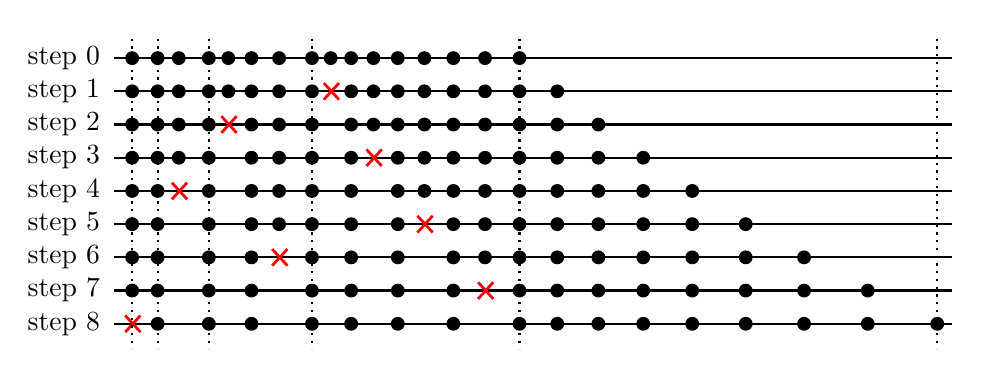
\begin{tikzpicture}[y=1pt, x=1pt,yscale=-1, inner sep=0pt, outer sep=0pt]
    \def\linespread{\baselineskip}
    \foreach \i in {0,1,2,...,8} {
      \path[shift={(0,0)}, draw=black, line join=miter, line cap=butt, line width=0.8pt]
        (0,\i * \linespread) node[left=5] {step \i} -- (303, \i * \linespread) ;
    }
    \foreach \x in {9.086718622889968, 18.28737691914821, 25.94320242291756, 36.80406189100548, 43.83609267359075, 52.211710397032434, 62.18762978904628, 74.06961521412411, 80.83661709068994, 88.22185242594281, 96.28180304394778, 105.07811094961241, 114.67804976293608, 125.155039223504, 136.58920670012435, 149.068} {
      \path[fill=black]
              (\x,0)arc(0.000:180.000:2.500)arc(-180.000:0.000:2.500) -- cycle;
    }
    \draw (149.068,0) node [above=10] {};

    \foreach \x in {9.086718622889968, 18.28737691914821, 25.94320242291756, 36.80406189100548, 43.83609267359075, 52.211710397032434, 62.18762978904628, 74.06961521412411, 88.22185242594281, 96.28180304394778, 105.07811094961241, 114.67804976293608, 125.155039223504, 136.58920670012435, 149.068, 162.6868561641611} {
      \path[fill=black]
              (\x,\linespread )arc(0.000:180.000:2.500)arc(-180.000:0.000:2.500) -- cycle;
    }
    \foreach \x in {9.086718622889968, 18.28737691914821, 25.94320242291756, 36.80406189100548, 52.211710397032434, 62.18762978904628, 74.06961521412411, 88.22185242594281, 96.28180304394778, 105.07811094961241, 114.67804976293608, 125.155039223504, 136.58920670012435, 149.068, 162.6868561641611, 177.549931364065} {
      \path[fill=black]
              (\x,2*\linespread)arc(0.000:180.000:2.500)arc(-180.000:0.000:2.500) -- cycle;
    }
    \foreach \x in {9.086718622889968, 18.28737691914821, 25.94320242291756, 36.80406189100548, 52.211710397032434, 62.18762978904628, 74.06961521412411, 88.22185242594281, 105.07811094961241, 114.67804976293608, 125.155039223504, 136.58920670012435, 149.068, 162.6868561641611, 177.549931364065, 193.7708974815676} {
      \path[fill=black]
              (\x,3*\linespread)arc(0.000:180.000:2.500)arc(-180.000:0.000:2.500) -- cycle;
    }
    \foreach \x in {9.086718622889968, 18.28737691914821, 36.80406189100548, 52.211710397032434, 62.18762978904628, 74.06961521412411, 88.22185242594281, 105.07811094961241, 114.67804976293608, 125.155039223504, 136.58920670012435, 149.068, 162.6868561641611, 177.549931364065, 193.7708974815676, 211.47381146446045} {
      \path[fill=black]
              (\x,4*\linespread)arc(0.000:180.000:2.500)arc(-180.000:0.000:2.500) -- cycle;
    }
    \foreach \x in {9.086718622889968, 18.28737691914821, 36.80406189100548, 52.211710397032434, 62.18762978904628, 74.06961521412411, 88.22185242594281, 105.07811094961241, 125.155039223504, 136.58920670012435, 149.068, 162.6868561641611, 177.549931364065, 193.7708974815676, 211.47381146446045, 230.79406410635147} {
      \path[fill=black]
              (\x,5*\linespread)arc(0.000:180.000:2.500)arc(-180.000:0.000:2.500) -- cycle;
    }
    \foreach \x in {9.086718622889968, 18.28737691914821, 36.80406189100548, 52.211710397032434, 74.06961521412411, 88.22185242594281, 105.07811094961241, 125.155039223504, 136.58920670012435, 149.068, 162.6868561641611, 177.549931364065, 193.7708974815676, 211.47381146446045, 230.79406410635147, 251.87941550709863} {
      \path[fill=black]
              (\x,6*\linespread)arc(0.000:180.000:2.500)arc(-180.000:0.000:2.500) -- cycle;
    }
    \foreach \x in {9.086718622889968, 18.28737691914821, 36.80406189100548, 52.211710397032434, 74.06961521412411, 88.22185242594281, 105.07811094961241, 125.155039223504, 149.068, 162.6868561641611, 177.549931364065, 193.7708974815676, 211.47381146446045, 230.79406410635147, 251.87941550709863, 274.8911251329348} {
      \path[fill=black]
              (\x,7*\linespread)arc(0.000:180.000:2.500)arc(-180.000:0.000:2.500) -- cycle;
    }
    \foreach \x in {18.28737691914821, 36.80406189100548, 52.211710397032434, 74.06961521412411, 88.22185242594281, 105.07811094961241, 125.155039223504, 149.068, 162.6868561641611, 177.549931364065, 193.7708974815676, 211.47381146446045, 230.79406410635147, 251.87941550709863, 274.8911251329348, 300.0051851189134} {
      \path[fill=black]
              (\x,8*\linespread)arc(0.000:180.000:2.500)arc(-180.000:0.000:2.500) -- cycle;
    }

    \draw (300.00518511, 8*\linespread) node [below=10pt] {};

    \foreach \i/\x in {1/80.8366170907, 2/43.8360926736, 3/96.2818030439, 4/25.9432024229, 5/114.678049763, 6/62.187629789, 7/136.5892067, 8/9.08671862289} {
      \path[draw=red, line width = 1pt] 
        (\x - 5, \i * \linespread - 3) -- (\x + 0.5 , \i  * \linespread + 3);
      \path[draw=red, line width = 1pt]
        (\x - 5, \i * \linespread + 3) -- (\x + 0.5, \i  * \linespread - 3);
    }
    \foreach \x in {9.086718622889968, 18.28737691914821, 36.80406189100548, 74.06961521412411, 149.068, 300.0051851189134} {
      \path[draw=black, dotted, line width = 0.8pt]
        (\x -2.5, -7) -- (\x -2.5, 8*\linespread + 9);
    }
\end{tikzpicture}
\caption{One period of the algorithm \AlgJakub\ for . Note that, recursively, checkpoints are removed twice as often from the right half of the initial setting \LV{(at steps  where ) }as from the second quarter. }
\label{fig:jakubs_algorithm_movement}
\end{figure}

\subsection{Discrepancy Analysis} 
We now bound the largest discrepancy encountered during one period, i.e.,

\SV{

  By Lemma~\ref{lem:only_new_intervals}, we only have to consider intervals newly created by insertion and deletion at any step. We do this exemplarily for the intervals from insertion.
}\LV{

  We first compute the maximum and later multiply with the factor .
  By Lemma~\ref{lem:only_new_intervals}, we only have to consider intervals newly created by insertion and deletion at any step.

}
\paragraph{Intervals from Insertion:}
We \LV{first }compute the discrepancy of the interval newly added at time , . Its length is , so its discrepancy \LV{(without the factor ) }is
  
  where the second equality holds because of \eqref{eq:newti} if  or \eqref{eq:tialpha} if .

  Using  for  yields a bound on the discrepancy of 
  
 \SV{ Since we choose , we obtain a discrepancy of roughly , and the error term can easily be seen to be bounded by . }

\LV{

\paragraph{Deleting :} 
We show similar bounds for the intervals we get from deleting an old checkpoint. We first analyze the deletion of ---this case is different from the general one, since  has no predecessor. Note that  is deleted at time . The deletion of  creates the interval . This interval has discrepancy

since we choose . Hence, this discrepancy is dominated by the one we get from newly inserted intervals.


\paragraph{Other Intervals from Deletion:} 
It remains to analyze the discrepancy of the intervals we get from deletion in the general case, i.e., at some time , . At this time we delete checkpoint , so we create the interval  of discrepancy

Let , so that  is the largest power of 2 dividing , and . Then  by \eqref{eq:tialpha}, and a similar statement holds for , yielding

Using \eqref{eq:tiinterpol} we get . Comparing this with the respective terms for  and  yields

By elementary means one can show that the function , , is convex on . Since convex functions have their maxima at the boundaries of their domain, and since by above equation  can be expressed using  (for  and ), we see that  is maximal at (one of) the boundaries of . Recall that we treated  separately, and observe that the largest power of 2 dividing ,  is at most . Hence, we have  and 

We simplify using  and  to get

The first term is already of the desired form. For the second one, note that setting  we would get a discrepancy of . We get a better bound by choosing

with .
Then the second bound on  from above becomes

The particular choice of  allows to bound the derivative of  for  from above by 

Hence, we can upper bound 

Thus, in total the second bound on  from inequality~(\ref{eq:jakubsqi}) becomes 

Since , this becomes 


\paragraph{Overall discrepancy:} 
In total, we can bound the discrepancy  of our algorithm (now including the factor of ) by

Using  and 

this bound can be simplified to

which proves Theorem~\ref{thm:algjacub}.
}
